\documentclass[10pt]{article}
\usepackage{mathtools}
\usepackage{amsfonts}
\usepackage{pifont}
\usepackage{pgfplots}
\pgfplotsset{compat=newest}
\newcommand*{\perm}[2]{{}^{#1}\!P_{#2}}%
\author{BM Corser}
\title{Calculus 2 Assignment 1}
\date{}
\begin{document}
    \maketitle 
    \begin{enumerate}
        \item Because $f(0) = 0$, there can be no constant component to the
            function. Because the domain and codomain are $\mathbb{R}$, $f(x)$
            cannot be $ax^{\tfrac{1}{b}}$ where $b > 1$ because $f(x) \notin
            \mathbb{R}$ when $x$ is negative. Also the function cannot be of
            the form $\frac{a}{bx}$ because $f(0) \notin \mathbb{R}$. The
            function $f$ must then be of the form $f(x) = ax^b$ where $b > 1$,
            $f(x) = \frac{x^a}{b}$ where $a > 1$ or the null case $f(x) = 0$.
        \begin{enumerate}
            \item To meet the condition $f(x) \leq x \ \forall \ x \in
                \mathbb{R}$, then the only possible forms $f(x)$ can take are
                $f(x) = x$ for which $\frac{df}{dx} = 1$ and $f(x) = 0$ for
                which $\frac{df}{dx} = 0$. In both these cases $\frac{df}{dx}
                \leq 1$ and as such the statement is true.
            \item Let $\frac{df}{dx} = \frac{1}{3}$, then
                $\int\frac{df}{dx} = f(x) = \frac{x}{3} + c$. Since we have
                established our $f$ cannot have a constant component, $c = 0$.
                Now let $x = -1$, then $f(x) = -\frac{1}{3} > x$ which is a
                counterexample, proving the statement false.
        \end{enumerate}
    \item Let $f(x) = x + 2$ and $g(x) = 2x + 1$, then
        \begin{align*}
            f(g(x)) &\neq g(f(x)) \\
            (2x + 1) + 2 &\neq 2(x + 2) + 1 \\
            2x + 3 &\neq 2x + 5 \\
        \end{align*}
        also
        \begin{align*}
            \frac{d}{dx}\Big(f\big(g(x)\big)\Big) &= \frac{d}{dx}\Big(g\big(f(x)\big)\Big) \\
            \frac{d}{dx}(2x + 3) &= \frac{d}{dx}(2x + 5) \\
            2 &= 2 \\
        \end{align*}
        \pagebreak
    \item Given
        \begin{align*}
        \lim_{x \to 0}\frac{f(x)}{x} = 7
        \end{align*}
        and since when 
        \begin{align*}
            \lim_{x \to a}g(x) = l
        \end{align*}
        and 
        \begin{align*}
            \lim_{x \to a}h(x) = m
        \end{align*}
        then
        \begin{align*}
        lim_{x \to a}h(x)\cdot\lim_{x \to a}\frac{g(x)}{h(x)} = m\cdot\frac{l}{m} = l
        \end{align*}
        and
        \begin{align*}
            \lim_{x \to 0} \frac{f(x)}{x} &= 7 \\
            \lim_{x \to 0}f(x) &= 7 \cdot \lim_{x \to 0} x \\
            \lim_{x \to 0}f(x) &= 0 \\
        \end{align*}
        and since for continuous functions $\lim_{x \to a}p(x) = p(a)$
        \begin{align*}
            f(0) &= 0 \\
        \end{align*}
        and since for $x = 0$
        \begin{align*}
            \frac{df}{dx} &= \lim_{h \to 0} \frac{f(x + h) - f(x)}{h} \\
            \frac{df}{dx} &= \lim_{h \to 0} \frac{f(h)}{h} \\
        \end{align*}
            now let $h =x$ then clearly $f'(0) = 7$. Another function that
            satisfies the conditions presented here is $f(x) = x^{9000} + 7x$

    \item Let $b = \frac{1}{3}$ and $b = 9$, then
        \begin{enumerate}
            \item
                \begin{align*}
                    \lim_{x \to \infty} \frac{x + 9}{\tfrac{1}{3}x + 1} &= \frac{x}{\tfrac{1}{3}x} \\
                    &= \frac{3x}{x} \\
                    &= 3 \\
                \end{align*}
                and
                \begin{align*}
                    \lim_{x \to 0} \frac{x + 9}{\tfrac{1}{3}x + 1} &= \frac{9}{1} \\
                    &= 9 \\
                \end{align*}
                also
            \item $U = \mathbb{R} \setminus \{3\}$
        \end{enumerate}
    \item
        \begin{enumerate}
            \item $f(x, y) = x^2 - 2x + y^2 - 4y + 5 = (x - 1)^2 + (y - 2)^2$

                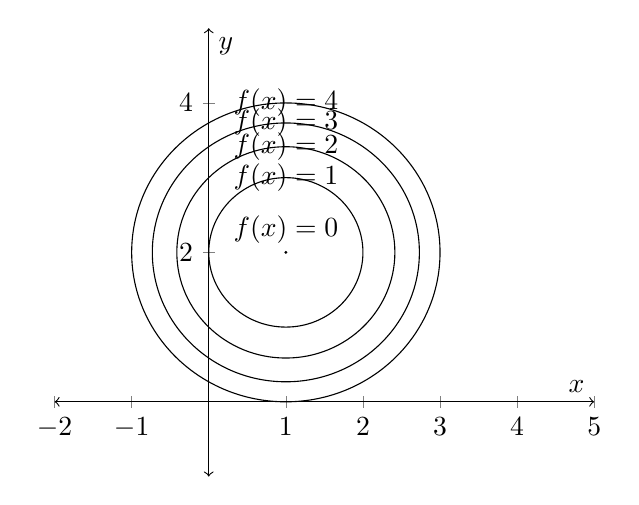
\begin{tikzpicture}
                    \begin{axis}[
                        xmin=-2,xmax=5,
                        ymin=-1,ymax=5,
                        axis x line=middle,
                        axis y line=middle,
                        axis line style=<->,
                        xlabel={$x$},
                        ylabel={$y$},
                        ]
                        \draw [] (axis cs: 1,2) circle [radius=0.01];
                        \draw [] (axis cs: 1,2) circle [radius=1];
                        \draw [] (axis cs: 1,2) circle [radius=sqrt(2)];
                        \draw [] (axis cs: 1,2) circle [radius=sqrt(3)];
                        \draw [] (axis cs: 1,2) circle [radius=sqrt(4)];
                        \node at (axis cs: 1,2.3) {$f(x) = 0$};
                        \node at (axis cs: 1,3) {$f(x) = 1$};
                        \node at (axis cs: 1,{2 + sqrt(2)}) {$f(x) = 2$};
                        \node at (axis cs: 1,{2 + sqrt(3)},2) {$f(x) = 3$};
                        \node at (axis cs: 1,4) {$f(x) = 4$};
                    \end{axis}
                \end{tikzpicture}

                It doesn't make sense to plot contours for values of $a < 0$
                because there is no circle with a smaller radius than 0.
            \item
                \begin{align*}
                    f(x, y) &= x^2 - 2x + y^2 - 4y + 5 \\
                    f_x &= 2x - 2 \\
                    f_y &= 2y - 4 \\
                \end{align*}
                Let $a = 0$ and $b = 2$. The equation of  tangent plane passing
                through the point $P = (a, b, f(a, b))$ is
                \begin{align*}
                    f_x(a, b)(x - a) + f_y(a, b)(y - b) + f(a, b) - z = 0 \\
                \end{align*}
                \begin{align*}
                    f_x(a, b) &= -2 \\
                    f_y(a, b) &= 0 \\
                    f(a, b) &= 1 \\
                \end{align*}
                \begin{align*}
                    -2x + 1 - z &= 0 \\
                    z &= 1-2x
                \end{align*}
            \item 
                \begin{align*}
                    \nabla f = \left(\!
                        \begin{array}{c}
                        2x -2 \\
                        2y -4
                        \end{array}
                    \!\right)
                \end{align*}
        \end{enumerate}
        \item 
            \begin{align*}
                \Pi = 2x +y + 3z &= 6 \\
                z &= 2-\frac{2x}{3} - \frac{y}{3}\\
            \end{align*}
            setting $z = 0$
            \begin{align*}
                2-\frac{2x}{3} - \frac{y}{3} &= 0 \\
                y &= 6 - 2x \\
            \end{align*}
            bounds are
            \begin{align*}
                0 \leq x \leq 3 \\
                0 \leq y \leq 6 - 2x
            \end{align*}
            let $D$ be the bounded area
            \begin{align*}
                \int\int_D\Pi dA &= \int_0^3\int_0^{6-2x} 2-\frac{2x}{3} - \frac{y}{3} dydx \\
                &= \int_0^3\Big[2y-\frac{2xy}{3} - \frac{y^2}{6}\Big]_0^{6-2x} dx \\
                &= \int_0^3 2(6-2x)-\frac{2x(6-2x)}{3} - \frac{(6-2x)^2}{6} dx \\
                &= 6
            \end{align*}
            setting bounds for $dx$ inner
            \begin{align*}
                0 \leq y \leq 6 \\
                0 \leq x \leq 3 - \frac{y}{2}
            \end{align*}
            \begin{align*}
                \int\int_D\Pi dA &= \int_0^6\int_0^{3-\frac{y}{2}} 2-\frac{2x}{3} - \frac{y}{3} dxdy \\
                &= \int_0^6\Big[2x-\frac{2x^2}{6} - \frac{xy}{3}\Big]_0^{3-\frac{y}{2}} dy \\
                &= \int_0^6 2(3-\frac{y}{2})-\frac{2(3-\frac{y}{2})^2}{6} - \frac{(3-\frac{y}{2})y}{3}  dy \\
                &= 6
            \end{align*}
    \end{enumerate}
\end{document}
